\documentclass[]{beamer}
\usetheme{CambridgeUS} % theme
\usepackage[english]{babel}
\usepackage[utf8]{inputenc}
\usepackage[T1]{fontenc}
\usepackage{fancyhdr}
\usepackage{float}
\usepackage{graphicx}
\usepackage{wrapfig}
\usepackage{amssymb}
\usepackage{amsmath}
\usepackage{mathtools}
\usepackage{amsfonts}
\usepackage{tikz}
\setbeamercovered{transparent} % \pause text visibility
\usepackage{mathtools}

%------------------------------ TITLE PAGE DECLARATION
\title[]{\textsc{Implementation and performance analysis of WiMAX 802.16 LDPC Code}}
\subtitle[]{Channel Coding Final Project}
\author[]{Tommaso Zugno}
\date[]{15/12/2017}
%\institute[]{Università degli Studi di Padova\\ Dipartimento di Ingegneria dell'Informazione}
%\logo{
\includegraphics[width=1cm]{figure1/logo_unipd}}
%------------------------------ /TITLE PAGE DECLARATION

\begin{document}
\transduration{1}
\frame{\titlepage} %------------------------------ TITLE PAGE
%\section*{}
\section{   }

%\subsection{}
\begin{frame}
\transwipe[direction=0]
\frametitle{Outline}

\end{frame}


\begin{frame}
\transwipe[direction=0]
\frametitle{WiMAX Technology}
WiMAX (Worldwide Interoperability for Microwave Access) is \textit{a standards-based technology enabling the delivery of last mile wireless broadband access as an alternative to cable and DSL} \footnote{\url{www.WiMAXforum.org/technology/}} .

\vspace{0.3cm}
WiMAX is based upon std. IEEE 802.16e-2005 which provides multiple PHY and MAC options.

\begin{columns}
		\column{0.4\textwidth}
			\begin{figure}
				\centering
					\includegraphics[width=2.5cm]{figure1/WiMAX}
			\end{figure}
		\column{0.4\textwidth}
			\begin{figure}
				\centering
					
\includegraphics[width=2.5cm]{figure1/wirelessman}
			\end{figure}
	\end{columns}
\centering
\end{frame}


%\subsection{SLIDE 3}
\begin{frame}
\transwipe[direction=0]
\frametitle{Channel coding in WirelessMAN-OFDMA PHY layer}
Channel coding procedure:

\begin{center}
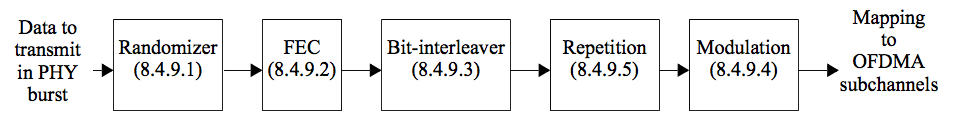
\includegraphics[width=10cm]{figure1/procedure}
\end{center}

The standard specifies different FEC options:
\begin{itemize}
\item Convolutional Coding (CC)
\item Convolutional Turbo Coding (CTC)
\item Block Turbo Coding 
\item \textbf{Low Density Parity Check codes}
\end{itemize}

\end{frame}

\begin{frame}
\transwipe[direction=0]
\frametitle{LDPC codes}
The standard specifies a LDPC code for each combination of rate $R$ and codeword length $n$. There are:
\begin{itemize}
\item 6 possible rates (1/2, 2/3A, 2/3B, 3/4A, 3/4B, 5/6)
\item 19 possible codeword lengths
\end{itemize}

\vspace{0.5cm}

We implemented in Matlab the encoder/decoder couple for some codes. In particular we considered:
%In this implementation we considered:
\begin{itemize}
\item 4 different rates (1/2, 2/3B, 3/4A, 5/6)
\item 3 different codeword lengths (576, 1344, 2304 bits)
\end{itemize}

%\vspace{0.3cm}

%The implementation is done in \texttt{Matlab}.
\end{frame}

%\subsection{SLIDE 4}
\begin{frame}
\transwipe[direction=0]
\frametitle{LDPC codes}
Each code in the set of LDPC codes is specified by a parity check matrix $H$ of size $m\times n$.

$H$ is defined as:
\begin{equation*}
H = 
	\begin{bmatrix}
		P_{0,0}  & P_{0,1} & \dots & P_{0,n_b-1}\\
		P_{1,0} & P_{1,1}  & \dots & P_{1,n_b-1} \\
		\vdots & \vdots & & \vdots \\
		P_{m_b-1,0} & P_{m_b-1,1} & \dots & P_{m_b-1,n_b-1}
	\end{bmatrix}
\end{equation*}

where $P_{i,j}$ is a $z\times z$ permutation matrices or a $z\times z$ zero matrix with $z = \frac{n}{n_b} = \frac{m}{m_b}$ and $n_b = 24$. 

The permutations used are circular right shifts.

\end{frame}


\begin{frame}
\transwipe[direction=0]
\frametitle{LDPC codes}
$H$ is expanded from a base model matrix $H_{bm}$ of size $m_b\times n_b$:
\begin{itemize}
\item each positive entry $p(i,j)$ is replaced with a $P_{i,j}$ matrix with circular shift size equal to $p(i,j)$
\item each blank or negative entry p(i,j) is replaced with a $P_{i,j}$ zero matrix
\end{itemize}
\vspace{0.3cm}
The standard defines $H_{bm}$ for the largest codeword length ($n = 2304$) of each code rate. $H_{bm}$ for a different codeword length $n'$ is obtained by scaling the shift sizes proportionally
	\begin{equation*}
		p'(i,j) =  \Bigg \{
				\begin{array}{rl}
					p(i,j) & p(i,j) \leq 0 \vspace{0.3cm}\\
					
					\left\lfloor\frac{p(i,j)z_f}{z_0} \right\rfloor & p(i,j) > 0 \\
				\end{array}
	\end{equation*}
where $z_0 = \frac{2304}{n_b}$ and $z_f = \frac{n'}{n_b}$.
\end{frame}

\begin{frame}
\transwipe[direction=0]
\frametitle{Encoding procedure}
For an efficient encoding, H is divided into the form:

\begin{equation*}
H = 
	\begin{bmatrix}
		A & B & T \\
		C & D & E \\
	\end{bmatrix}
\end{equation*}

We define: $M_1 = ET^{-1}A+C$, $M_2 = T^{-1}A$, $M_3 = T^{-1}B$.% \footnote{The matrices $M_1$. $M_2$ and $M_3$ are pre-computed and loaded at the begin of the simulation.}

\vspace{0.5cm}

Given the infoword $u$, we compute:
\begin{itemize}
\item $p_1^T = M_1u$
\item $p_2^T = M_2u + M_3p_1^T$
\end{itemize}
The corresponding codeword is $v = [u, p_1, p_2]$ 
\end{frame}


\begin{frame}
\transwipe[direction=0]
\frametitle{Encoder implementation}
Given the chosen values for the rate $R$ and codeword length $n$, the script \texttt{generate-matrices2.m}:
\begin{itemize}
\item generates the matrix $H$ using the corresponding base matrix $H_{bm}$
\item computes and saves the matrices $M_1$, $M_2$ and $M_3$
\end{itemize}

\vspace{0.5cm}

At the begin of each simulation, the matrices $M_1$, $M_2$ and $M_3$ are loaded and used during the encoding procedure.


\end{frame}


\begin{frame}
\transwipe[direction=0]
\frametitle{Decoding binary LDPC}
The decoding is performed using the Message Passing Algorithm (MPA) in the logarithmic domain. The MPA is based on this factor graph:

\begin{center}
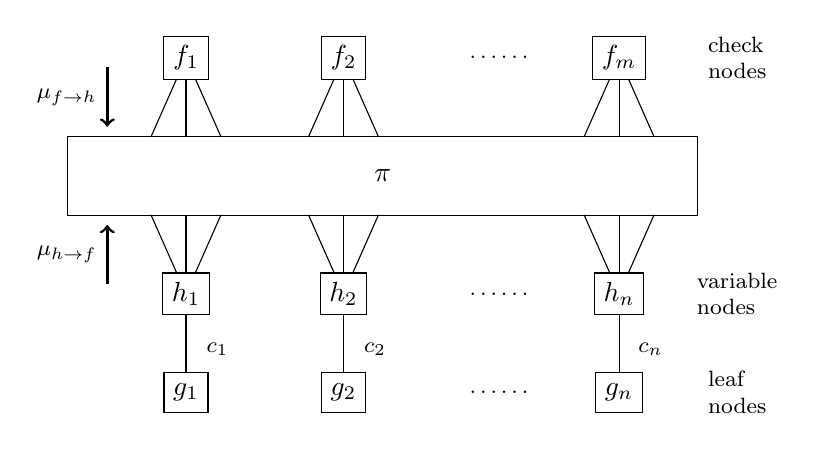
\begin{tikzpicture}[font=\footnotesize]
%\draw[help lines] (0 ,0) grid (8,6);
\draw [] (0,4) rectangle (8,5);
\node [font = \bfseries] at (4,4.5) {$\pi$};
\node at (5.5,6) {\dots\dots};
\node at (5.5,3) {\dots\dots};
\node at (5.5,1.75) {\dots\dots};
\node [align=left] at (8.5,6) {check \\ nodes \par};
\node [align=left] at (8.5,3) {variable \\ nodes \par};
\node [align=left] at (8.5,1.75) {leaf \\ nodes \par};
\node (f_1) [draw,minimum size = 0.5cm, font = \bfseries] at (1.5,6) {$f_1$};
\node (f_2) [draw,minimum size = 0.5cm, font = \bfseries] at (3.5,6) {$f_2$};
\node (f_n) [draw,minimum size = 0.5cm, font = \bfseries] at (7,6) {$f_m$};
\node (fl_1) [] at (1,4.87) {};
\node (fl_2) [] at (1.5,4.87) {};
\node (fl_3) [] at (2,4.87) {};
\node (fl_4) [] at (3,4.87) {};
\node (fl_5) [] at (3.5,4.87) {};
\node (fl_6) [] at (4,4.87) {};
\node (fl_7) [] at (6.5,4.87) {};
\node (fl_8) [] at (7,4.87) {};
\node (fl_9) [] at (7.5,4.87) {};
\node (h_1) [draw,minimum size = 0.5cm, font = \bfseries] at (1.5,3) {$h_1$};
\node (h_2) [draw,minimum size = 0.5cm, font = \bfseries] at (3.5,3) {$h_2$};
\node (h_n) [draw,minimum size = 0.5cm, font = \bfseries] at (7,3) {$h_n$};
\node (hl_1) [] at (1,4.13) {};
\node (hl_2) [] at (1.5,4.13) {};
\node (hl_3) [] at (2,4.13) {};
\node (hl_4) [] at (3,4.13) {};
\node (hl_5) [] at (3.5,4.13) {};
\node (hl_6) [] at (4,4.13) {};
\node (hl_7) [] at (6.5,4.13) {};
\node (hl_8) [] at (7,4.13) {};
\node (hl_9) [] at (7.5,4.13) {};
\node (g_1) [draw,minimum size = 0.5cm, font = \bfseries] at (1.5,1.75) {$g_1$};
\node (g_2) [draw,minimum size = 0.5cm, font = \bfseries] at (3.5,1.75) {$g_2$};
\node (g_n) [draw,minimum size = 0.5cm, font = \bfseries] at (7,1.75) {$g_n$};
\node (mufh1) at (0.5,6) {};
\node (mufh2) at (0.5,5) {};
\node (muhf1) at (0.5,3) {};
\node (muhf2) at (0.5,4) {};
\node (mugh1) at (0.5,1.8) {};
\node (mugh2) at (0.5,2.75) {};
\node (c1) at (1.9,2.3) {$c_1$};
\node (c2) at (3.9,2.3) {$c_2$};
\node (cn) at (7.4,2.3) {$c_n$};

\path
(f_1) edge node []{} (fl_1)
(f_1) edge node [left]{} (fl_2)
(f_1) edge node [left]{} (fl_3)
(f_2) edge node [left]{} (fl_4)
(f_2) edge node [left]{} (fl_5)
(f_2) edge node [left]{} (fl_6)
(f_n) edge node [left]{} (fl_7)
(f_n) edge node [left]{} (fl_8)
(f_n) edge node [left]{} (fl_9)
(h_1) edge node []{} (hl_1)
(h_1) edge node [left]{} (hl_2)
(h_1) edge node [left]{} (hl_3)
(h_2) edge node [left]{} (hl_4)
(h_2) edge node [left]{} (hl_5)
(h_2) edge node [left]{} (hl_6)
(h_n) edge node [left]{} (hl_7)
(h_n) edge node [left]{} (hl_8)
(h_n) edge node [left]{} (hl_9)
(g_1) edge node [left]{} (h_1)
(g_2) edge node [left]{} (h_2)
(g_n) edge node [left]{} (h_n)
(mufh1) edge [->, line width=1pt] node [left]{$\mu_{f\rightarrow h}$} (mufh2)
(muhf1) edge [->, line width=1pt] node [left]{$\mu_{h\rightarrow f}$} (muhf2);
%(mugh1) edge [->, line width=1pt] node [left]{$\mu_{g\rightarrow h}$} (mugh2);
\end{tikzpicture}
\end{center}

\end{frame}

\begin{frame}
\transwipe[direction=0]
%\frametitle{Leaf and variable nodes}

\begin{block}{Leaf nodes}
Under the hypothesis of equally probable input symbols, the messages from leaf to variable nodes are:

\begin{equation*}
g_l = - \frac{2r_l}{\sigma_w^2}
\end{equation*}
where $r_l$ is the l-th received symbol and  $\sigma_w^2$ is the noise variance.
\end{block}

\begin{block}{Variable nodes}
The update rule for the variable nodes is:

\begin{columns}
		\column{0.4\textwidth}
			\begin{equation*}
\mu_{h \rightarrow y} = \sum_{i} \mu_{x_i \rightarrow h}
\end{equation*}
		\column{0.4\textwidth}
			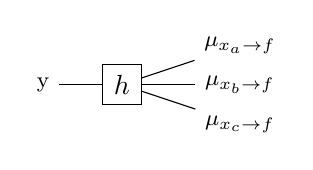
\begin{tikzpicture}[font=\footnotesize]
%\draw[help lines] (0 ,0) grid (8,6);
\node (f) [draw,minimum size = 0.5cm, font = \bfseries] at (0,0) {$h$};
\node (y) [] at (-1,0) {y};
\node (xa) [] at (1.5,0.5) {$\mu_{x_a \rightarrow f}$};
\node (xb) [] at (1.5,0) {$\mu_{x_b \rightarrow f}$};
\node (xn) [] at (1.5,-0.5) {$\mu_{x_c \rightarrow f}$};
\path
(f) edge node [above]{} (y)
(xa) edge node [left]{} (f)
(xb) edge node [left]{} (f)
(xn) edge node [left]{} (f);
\end{tikzpicture}
	\end{columns}

\end{block}

\end{frame}

\begin{frame}
\transwipe[direction=0]
%\frametitle{Check nodes}
\begin{block}{Check nodes}
The update rule for the check nodes is:

\begin{columns}
		\column{0.3\textwidth}
			\begin{center}
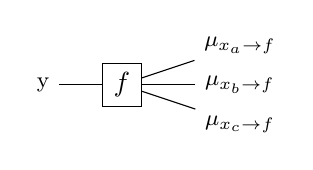
\begin{tikzpicture}[font=\footnotesize]
%\draw[help lines] (0 ,0) grid (8,6);
\node (f) [draw,minimum size = 0.5cm, font = \bfseries] at (0,0) {$f$};
\node (y) [] at (-1,0) {y};
\node (xa) [] at (1.5,0.5) {$\mu_{x_a \rightarrow f}$};
\node (xb) [] at (1.5,0) {$\mu_{x_b \rightarrow f}$};
\node (xn) [] at (1.5,-0.5) {$\mu_{x_c \rightarrow f}$};
\path
(f) edge node [above]{} (y)
(xa) edge node [left]{} (f)
(xb) edge node [left]{} (f)
(xn) edge node [left]{} (f);
\end{tikzpicture}
\end{center}

		\column{0.6\textwidth}
			\begin{equation*}
\mu_{f \rightarrow y} = \tilde \phi \bigg(\sum_i \tilde \phi \big( | \mu_{x_i \rightarrow f}| \big) \bigg) \prod_i sign( \mu_{x_i \rightarrow f})
\end{equation*}
	\end{columns}

\begin{columns}
		\column{0.4\textwidth}
		where:
			\begin{equation*}
				\tilde \phi = - \log \bigg ( tanh \bigg( \frac{1}{2}x\bigg) \bigg ) = \tilde \phi ^{-1}
			\end{equation*}
		\column{0.4\textwidth}
			\begin{figure}
				\centering
					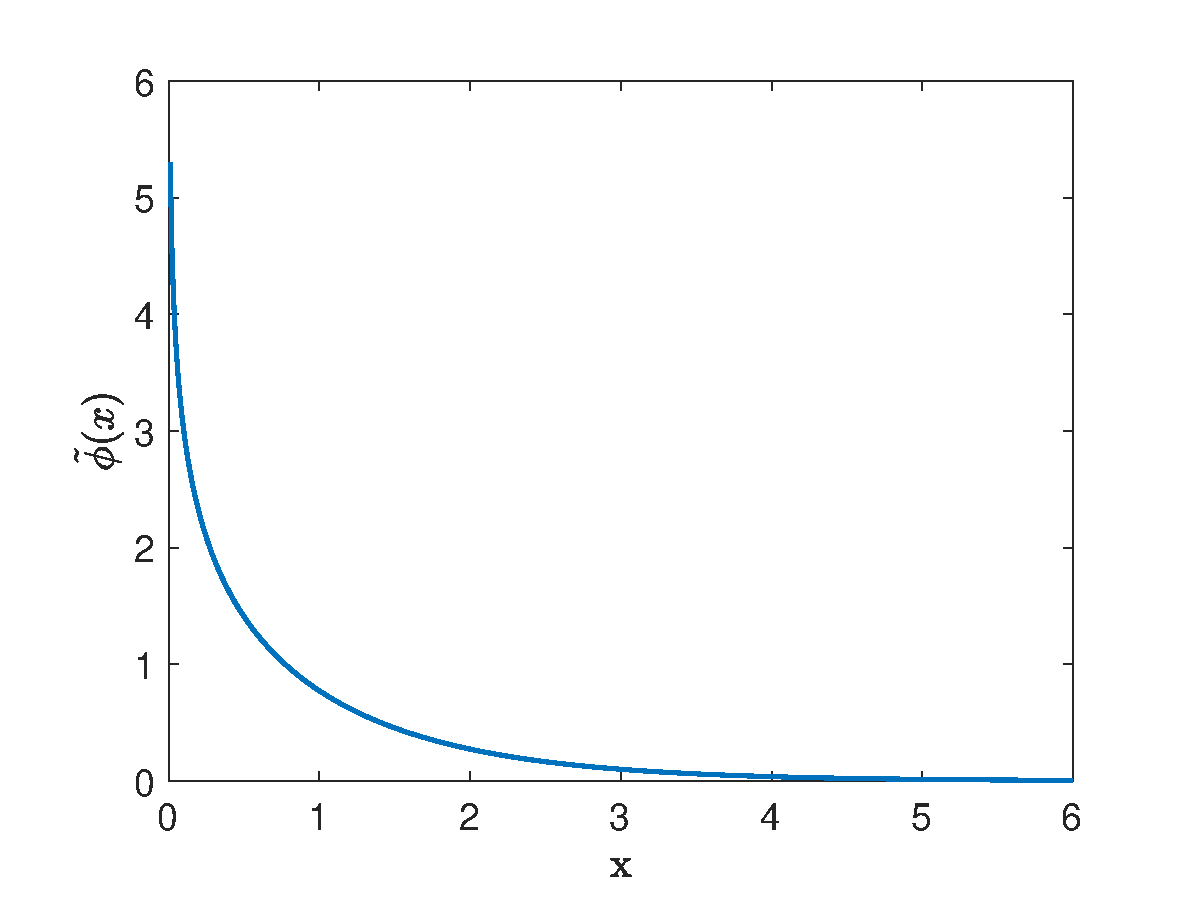
\includegraphics[width=5cm]{figure1/phi}
			\end{figure}
	\end{columns}



\end{block}

\end{frame}


\begin{frame}
\transwipe[direction=0]
\frametitle{Message Passing Algorithm}
\textbf{Initialization:} Messages $\mu_{h \rightarrow f}$ are initialized with the channel a-priori knowledge $g_l$.

\vspace{0.5cm}

\textbf{Schedule:}
\begin{enumerate}
\item run message passing on check nodes
\item run message passing on variable nodes
\item perform ongoing marginalization:
	\begin{equation*}
		\hat c_l = \bigg \{ \begin{array}{rl} 0 & ,\mu_{h_l \rightarrow c_l} + \mu_{g_l \rightarrow c_l} \geq 0 \\ 1 & ,otherwise \end{array}
	\end{equation*}
\item go back to step 1 until the maximum number of iterations is reached or a codeword is found
\end{enumerate} 

\end{frame}

\begin{frame}
\transwipe[direction=0]
\frametitle{Decoder implementation}
The decoder is implemented by the function \texttt{decode2.m} which outputs the estimate $\mathbf{\widehat u}$ of the transmitted infoword $\mathbf u$, given the received vector $\mathbf r$ and the noise variance $\sigma_w^2$.

\begin{itemize}
\item the vector \texttt{g} contains the messages exiting the leaf nodes and going upwards
\item the matrix \texttt{mu\_hf} contains the messages variable $\rightarrow$ check
\item the matrix \texttt{mu\_fh} contains the messages check $\rightarrow$ variable
\item the vector \texttt{mu\_hg} contains the messages exiting the leaf nodes and going downwards
\end{itemize}

%Vectorization is exploited in order to reduce the computation time.



\end{frame}

\begin{frame}
\transwipe[direction=0]
\frametitle{Decoder implementation}
\texttt{decode2.m} implements the Message Passing procedure described above:

\vspace{0.3cm}

%\begin{itemize}

%\item 
\textbf{Initialization:} compute \texttt{g} and initialize \texttt{mu\_hf}

 \textbf{while} max n of iterations is not reached AND codeword is not found
\begin{itemize}
\item update \texttt{mu\_fh}
	\begin{itemize}
		\item compute  $\tilde \phi$ (\texttt{mu\_hf}) and $sign$(\texttt{mu\_hf})
		\item sum the rows of $\tilde \phi$ (\texttt{mu\_hf}), multiply the rows of $sign$(\texttt{mu\_hf})
		\item for each outgoing branch, remove the contributes of the incoming message and compute \texttt{mu\_fh}
	\end{itemize}
\item update \texttt{mu\_hf} and \texttt{mu\_hg}
	\begin{itemize}
		\item sum the rows of \texttt{mu\_fh} and update \texttt{mu\_hg}
		\item add \texttt{g}, for each outgoing branch remove the contribute of the incoming message and update \texttt{mu\_hf}
	\end{itemize}
\item marginalize
\end{itemize}

\end{frame}

\begin{frame}
\transwipe[direction=0]
\frametitle{Decoder implementation}
The $\tilde \phi$ function is truncated to avoid over/underflow errors:
\begin{equation*}
\tilde \phi (x) = \Bigg\{
	\begin{array}{ll}
		12.5 & x < 10^{-5} \\
		-\log \big ( tanh \big( \frac{1}{2}x\big) \big ) & 10^{-5} \leq x < 50 \\
		0 & x \geq 50
	\end{array}
\end{equation*}

\end{frame}

\begin{frame}
\transwipe[direction=0]
\frametitle{Decoding BICM}
The BICM decoder was implemented by adding the conform nodes at the bottom of the LDPC factor graph. 

The bit-interleaving operation was not implemented.

\vspace{0.5cm}

The Message Passing schedule modifies into:
\begin{itemize}
	\item \textbf{Initialization:} compute the messages leaf $\rightarrow$ conform
	\item \textbf{Schedule:}
	\begin{enumerate}
		\item run message passing on the conform nodes
		\item update messages variable $\rightarrow$ check
		\item run message passing on the check nodes
		\item update messages variable $\rightarrow$ conform
		\item marginalize
	\end{enumerate}
\end{itemize}
\end{frame}

\begin{frame}
\transwipe[direction=0]
\frametitle{Decoding BICM}
The update rule for the conform nodes is:

\begin{equation*}
\mu_{\omega \rightarrow y} (y) = \log \left ( \frac{\sum\limits_{x_a, x_b, \dots} g(map(0,x_a,x_b,\dots)) e^{(1\oplus x_a)\mu_{x_a \rightarrow \omega}+(1\oplus x_b)\mu_{x_b \rightarrow \omega}+\dots}}{\sum\limits_{x_a, x_b, \dots} g(map(1,x_a,x_b,\dots)) e^{(1\oplus x_a)\mu_{x_a \rightarrow \omega}+(1\oplus x_b)\mu_{x_b \rightarrow \omega}+\dots}} \right)
\end{equation*}

\begin{center}
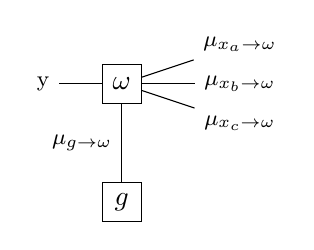
\begin{tikzpicture}[font=\footnotesize]
%\draw[help lines] (0 ,0) grid (8,6);
\node (f) [draw,minimum size = 0.5cm, font = \bfseries] at (0,0) {$\omega$};
\node (y) [] at (-1,0) {y};
\node (xa) [] at (1.5,0.5) {$\mu_{x_a \rightarrow \omega}$};
\node (xb) [] at (1.5,0) {$\mu_{x_b \rightarrow \omega}$};
\node (xn) [] at (1.5,-0.5) {$\mu_{x_c \rightarrow \omega}$};
\node (g) [draw,minimum size = 0.5cm, font = \bfseries] at (0,-1.5) {$g$};
\path
(f) edge node [above]{} (y)
(xa) edge node [left]{} (f)
(xb) edge node [left]{} (f)
(xn) edge node [left]{} (f)
(g) edge node [left] {$\mu_{g \rightarrow \omega}$} (f);
\end{tikzpicture}
\end{center}


\end{frame}

\begin{frame}
\transwipe[direction=0]
\frametitle{BICM decoder implementation}
The BICM decoder is implemented by the function \texttt{decodeBICM.m} which outputs the estimate $\mathbf{\widehat u}$ of the transmitted infoword $\mathbf{u}$ given the received vector $\mathbf{r}$ and the noise variance $\sigma_w^2$. 

\vspace{0.5cm}

The BICM decoder was implemented starting from \texttt{decode2.m}. The initialization and schedule was modified as described above to include the contribute of the conform nodes.
\end{frame}

\begin{frame}
\transwipe[direction=0]
\frametitle{main.m}
The script \texttt{main.m} runs a simulation campaign to test the performance of a code in terms of $P_{bit}$ vs $E_b/N_0$.

For each $E_b/N_0$ value to test, the simulation follows this schedule:
%\begin{itemize}
%\item \textbf{while} error threshold AND max num of packets are not reached
	\begin{enumerate}
		\item generate a random infoword $\mathbf{u}$
		\item encode $\mathbf{u}$ to obtain $\mathbf{c}$
		\item modulate $\mathbf{c}$ to obtain $\mathbf{c_{mod}}$
		\item add AWGN noise with variance $\sigma_w^2$ to obtain $\mathbf{r}$
		\item decode $\mathbf{r}$ to obtain $\mathbf{\widehat u}$
		\item compute the number of errors comparing $\mathbf{u}$ and $\mathbf{\widehat u}$
		\item go back to step 1 until the total number of errors or the number of transmitted packets reach the threshold
	\end{enumerate}
%\end{itemize}

\end{frame}

\begin{frame}
\transwipe[direction=0]
\frametitle{main.m}
%\begin{itemize}
Each bit of the infoword $\mathbf{u}$ is randomly generated using uniform probability distribution.

\vspace{0.5cm}

The modulation is performed by the function \texttt{modulate.m}. It supports 4 different modulation schemes (BPSK, QPSK, 16-QAM, 64-QAM). All the schemes have unitary average constellation energy.
A Gray coded bit-assignment is used.% in all the schemes. 

\vspace{0.5cm}

AWGN noise is generated with unitary variance and then scaled by $\sigma_w$. The noise variance is computed as $\sigma_w^2 = \frac{1}{\Gamma}$. %In the case of BICM, each noise component (real and complex) is scaled by $\frac{\sigma_w}{\sqrt{2}}$
%\end{itemize}
\end{frame}

\begin{frame}
\transwipe[direction=0]
\frametitle{Results}
Performance of binary LDPC ($n = 576$, $R = 5/6$) for different number of iterations.
\begin{center}
\begin{figure}
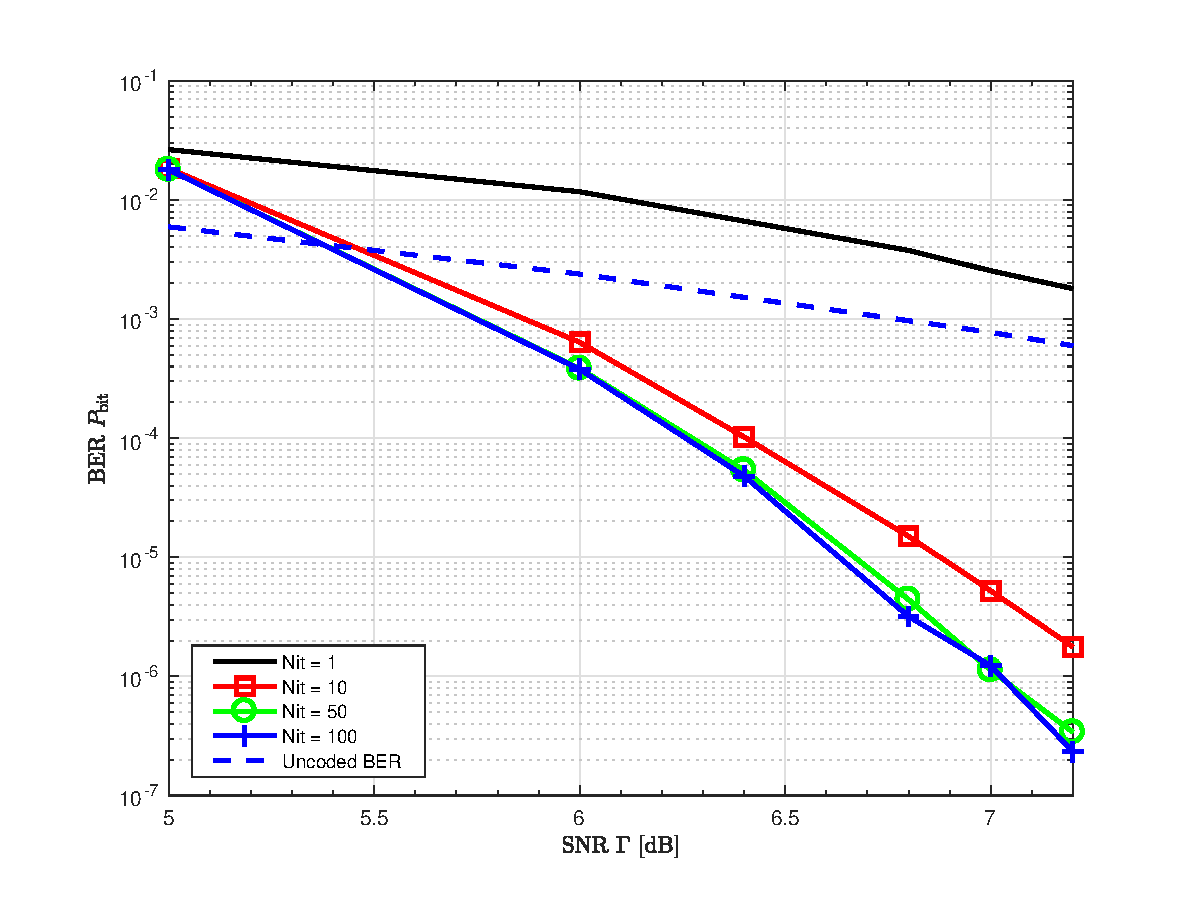
\includegraphics[width=9.8cm, trim={0 0 0 0.9cm},clip]{figure1/Nit}
%\caption{ciao}
\end{figure}
\end{center}

\end{frame}

\begin{frame}
\transwipe[direction=0]
\frametitle{Results}
Performance of binary LDPC ($n = 576$, $N_{it} = 50$) for different rates.
\begin{center}
\begin{figure}
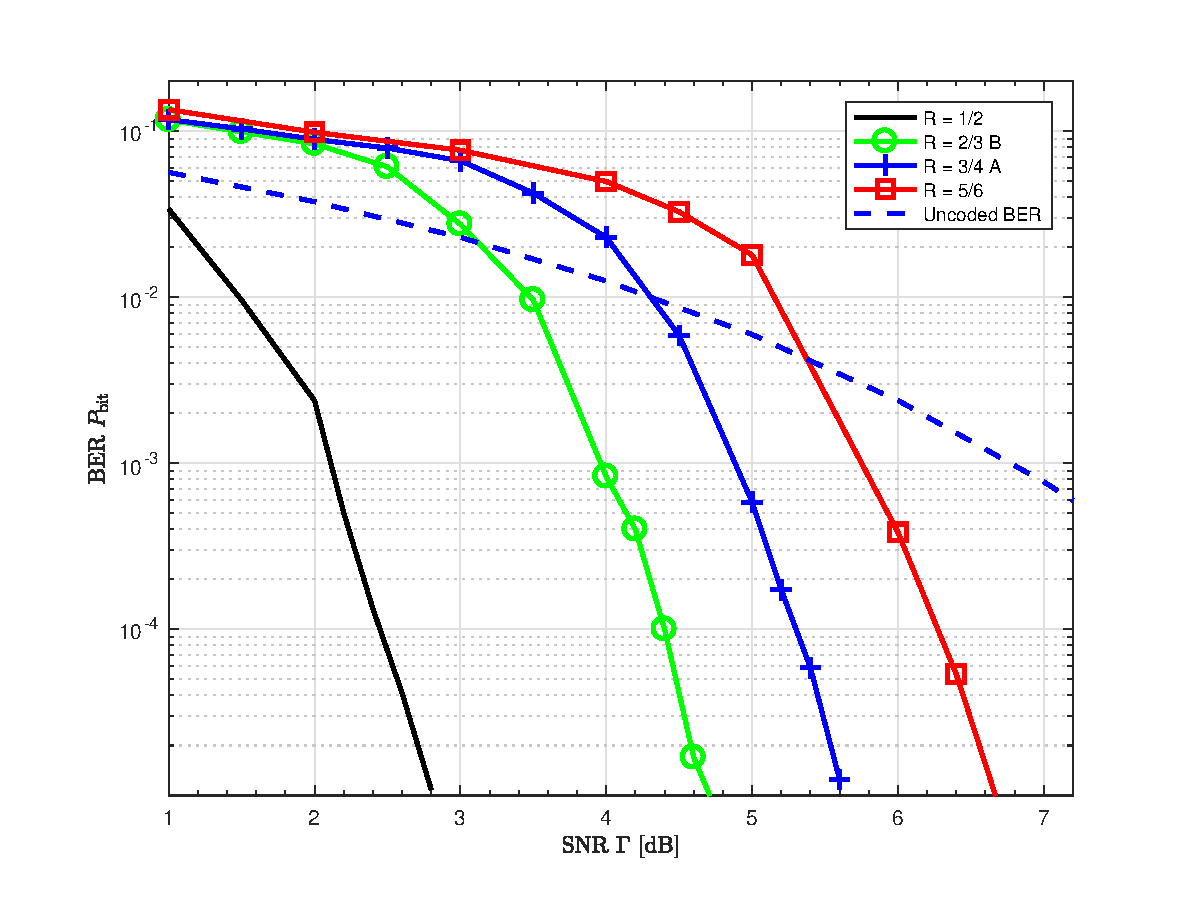
\includegraphics[width=9.8cm, trim={0 0 0 0.3cm},clip]{figure1/r}
%\caption{ciao}
\end{figure}
\end{center}

\end{frame}

\begin{frame}
\transwipe[direction=0]
\frametitle{Results}
Performance of binary LDPC ($R = 3/4 A$, $N_{it} = 50$) for different codeword lengths.
\begin{center}
\begin{figure}
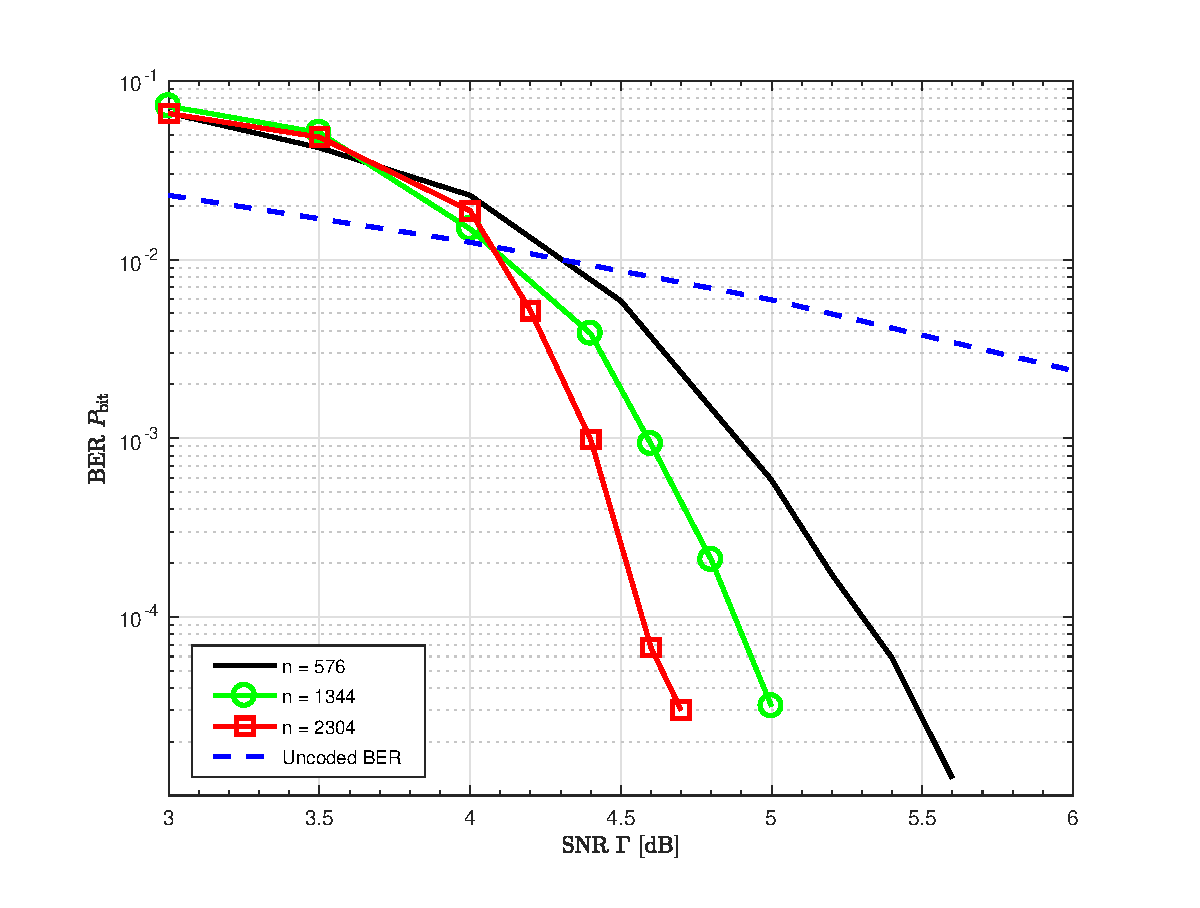
\includegraphics[width=9.8cm, trim={0 0 0 0.9cm},clip]{figure1/n}
%\caption{ciao}
\end{figure}
\end{center}
\end{frame}


\begin{frame}
\transwipe[direction=0]
\frametitle{Results}
Performance of BICM - LDPC ($n = 576$, $R = 5/6$, $N_{it} = 50$) for different modulation schemes.
\begin{center}
\begin{figure}
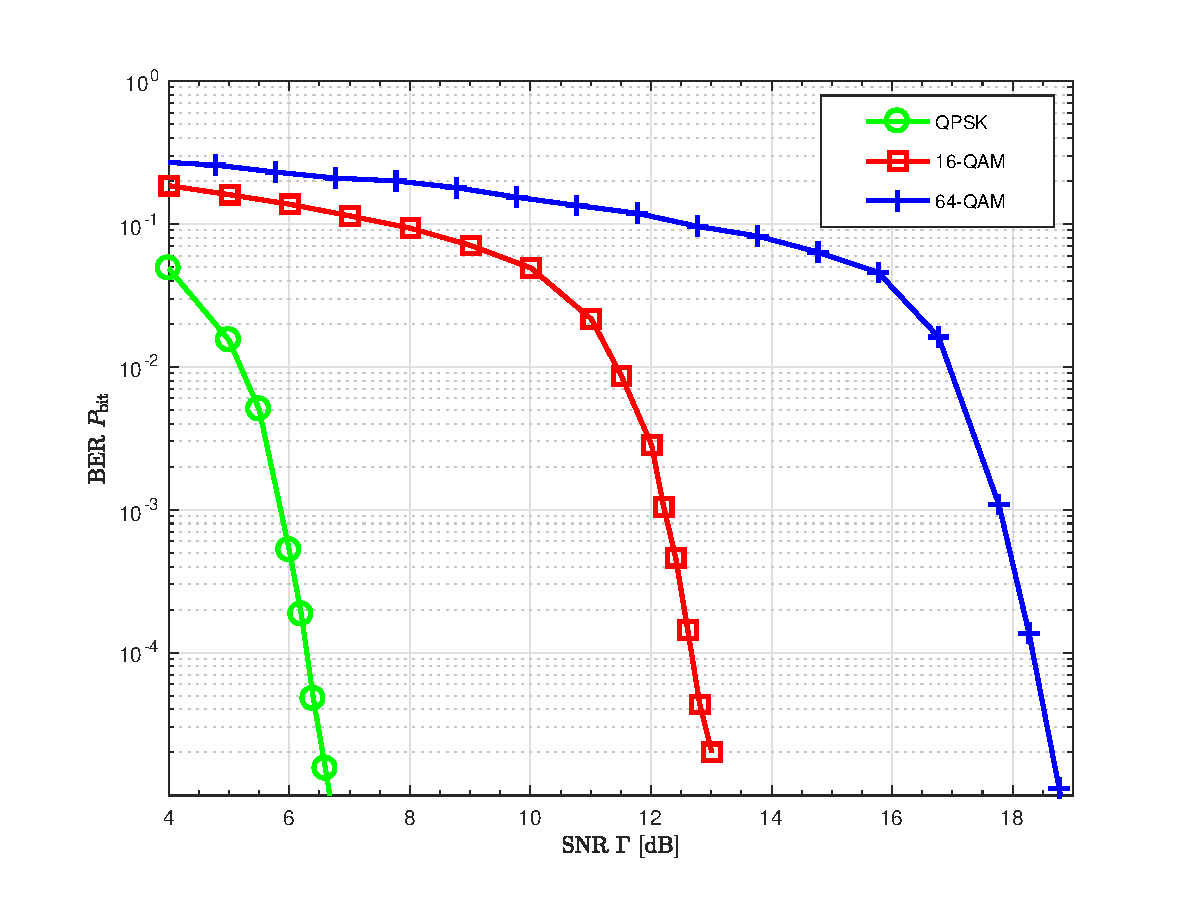
\includegraphics[width=9.8cm, trim={0 0 0 0.9cm},clip]{figure1/bicm}
%\caption{ciao}
\end{figure}
\end{center}

\end{frame}






\end{document}